\documentclass[a4paper,10pt]{article}
\usepackage[margin=2cm]{geometry}
\usepackage{tikz}
\usetikzlibrary{shapes.geometric, arrows.meta, positioning}

\pagestyle{empty}

\tikzstyle{node} = [rectangle, rounded corners=3pt, minimum width=4.2cm, minimum height=1.2cm, text centered, draw=black, fill=blue!10]
\tikzstyle{terminal} = [node, fill=green!20]
\tikzstyle{arrow} = [thick, ->, >=Stealth]

\begin{document}
	
\begin{center}
	\Large \textbf{LangGraph Execution Flow for Weather Forecast Assistant}
\end{center}

\vspace{0.5cm}

\begin{center}
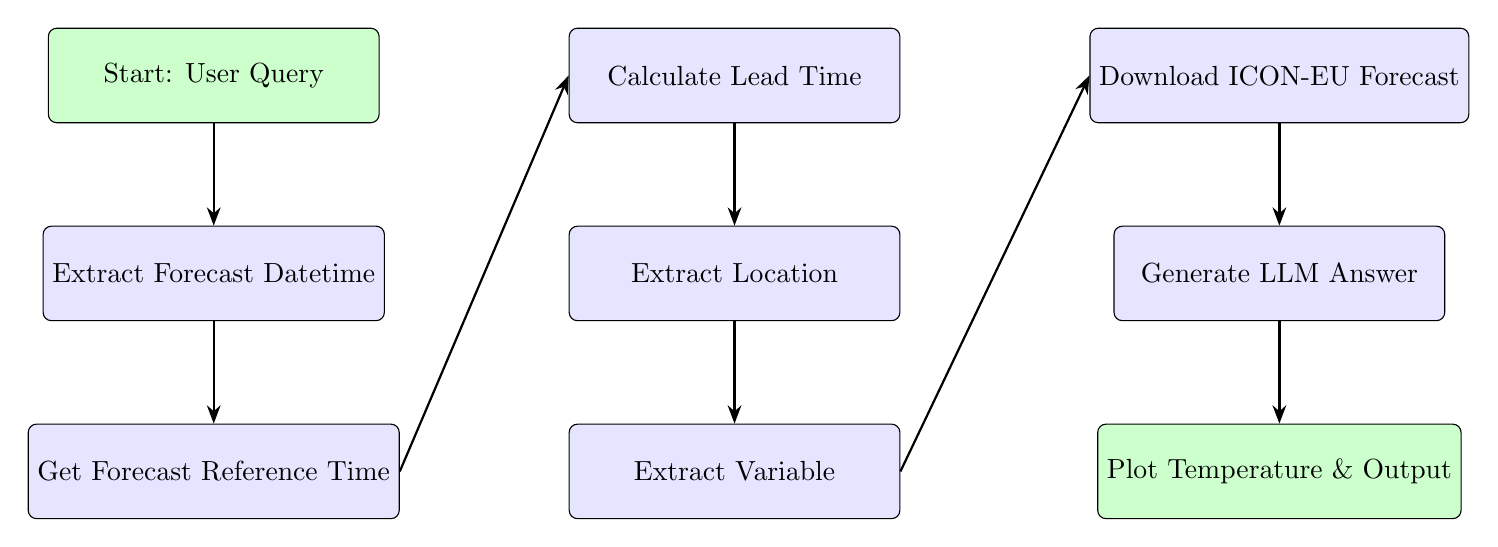
\begin{tikzpicture}[node distance=1.3cm and 2.4cm]
	
	% Column 1
	\node (start) [terminal] {Start: User Query};
	\node (datetime) [node, below=of start] {Extract Forecast Datetime};
	\node (ref) [node, below=of datetime] {Get Forecast Reference Time};

	% Column 2
	\node (leadtime) [node, right=of start] {Calculate Lead Time};
	\node (location) [node, below=of leadtime] {Extract Location};
	\node (variable) [node, below=of location] {Extract Variable};

	% Column 3
	\node (download) [node, right=of leadtime] {Download ICON-EU Forecast};
	\node (answer) [node, below=of download] {Generate LLM Answer};
	\node (plot) [terminal, below=of answer] {Plot Temperature \& Output};

	% Arrows column 1
	\draw [arrow] (start) -- (datetime);
	\draw [arrow] (datetime) -- (ref);

	% Link to column 2
	\draw [arrow] (ref.east) -- (leadtime.west);
	\draw [arrow] (leadtime) -- (location);
	\draw [arrow] (location) -- (variable);

	% Link to column 3
	\draw [arrow] (variable.east) -- (download.west);
	\draw [arrow] (download) -- (answer);
	\draw [arrow] (answer) -- (plot);

\end{tikzpicture}
\end{center}

\end{document}
